\chapter{Zpracování přirozeného jazyka}
V této práci bylo nezbytné zajistit, aby stroj byl schopen alespoň částečně porozumět lidsky psanému textu.
Přesně touto problematikou se zabývá oblast Zpracování přirozeného jazyka (Natural language processing~-~NLP)~\cite{link8}~\cite{link9},
 která kombinuje různé techniky, jako je lingvistika, informatika a umělá inteligence, s cílem zkoumat interakci mezi strojem a lidským jazykem.
S využitím poznatků z této oblasti je možné programovat počítače k zpracování a analýze velkých množství textových dat.
Tím se umožňuje počítačům porozumět kontextu v textu.
Zpracování přirozeného jazyka se zaměřuje na širokou škálu výzev, včetně rozpoznávání řeči, porozumění přirozenému jazyku a generování přirozeného jazyka.
Má bohatou historii a vyvinulo se mnoho technik pro zpracování přirozeného jazyka.
V této konkrétní práci je zvláště vhodná technika nazývaná Sentimentální analýza (Sentiment Analysis), která vychází z přirozeného zpracování jazyka.\@

\section{Sentimentální analýza}
Sentimentální analýza (Sentiment analysis)~\cite{link10} je jednou z nejčastěji používaných technik v oblasti zpracování přirozeného jazyka.\@
Je široce využívána pro řešení problémů spojených s určováním polarity textu, tj.\ zda je text pozitivní, neutrální nebo negativní.
Tato technika se aplikuje na různé typy textů, jako jsou dotazníky, komentáře, recenze a také na detekci strojového překladu, což je také cílem této práce.
Před použitím analýzy je však nezbytné předzpracovat text, na kterém chceme provádět detekci, a převést ho do formátu, který je srozumitelný pro modely.

\section{Metody analýzy textu}
Algoritmy strojového učení, jako jsou ty využívané při zpracování přirozeného jazyka, preferují jasně definovaná vstupní data pevné délky.
Proto je často potřeba přizpůsobit data tak, aby odpovídala požadovanému formátu.
To může zahrnovat osekávání nebo doplňování prázdnými hodnotami.
Tyto algoritmy nejsou schopny přímo pracovat s textem ve své původní podobě.
Z tohoto důvodu je nezbytné provést předzpracování lidského textu a převést jej na číselnou podobu, například pomocí vektorizace textu.
Existuje mnoho různých metod a technik, které slouží k tomuto účelu.

\section{One-hot kódování}
Metoda One-hot kódování (One-hot encoding) je základní technikou převodu textu do číselné podoby v oblasti zpracování přirozeného jazyka.\@
Tato metoda pracuje s tabulkou, nazývanou slovníkem, která mapuje jedinečná slova v textu na binární vektory.
Každé unikátní slovo ve větě je reprezentováno nulovým vektorem předem definované velikosti, a na pozici odpovídající konkrétnímu unikátnímu slovu je nastavena hodnota 1.
Tato hodnota indikuje přítomnost daného slova v číselném vektoru. Tímto způsobem je možné převést lidsky psané texty do číselné podoby, kterou následně mohou různé algoritmy zpracovávat.

\subsection{Nevýhody One-hot kódování}
Metoda One-hot~\ref{fig:One-hot encoding} kódování má významné omezení, kterým je značná neefektivnost pro velké množství unikátních slov.
Představme si větu obsahující tisíc slov.
Pro každé unikátní slovo v této větě by bylo potřeba vytvořit unikátní nulový vektor, kde pouze jedno místo by mělo hodnotu 1 pro reprezentaci konkrétního slova.
To znamená, že většina hodnot ve vektoru by byla nulová, což je značné plýtvání pamětí a výpočetních zdrojů.
Navíc, s přidáním každého nového slova se musí zvětšovat velikost všech vektorů ve slovníku a přidávat hodnoty 0, které nemají žádný význam.

Tento problém je jedním z důvodů, proč byly vyvinuty efektivnější metody reprezentace textu, jako je například vkládání slov (word embedding).

\begin{figure}[H]
	\centering
	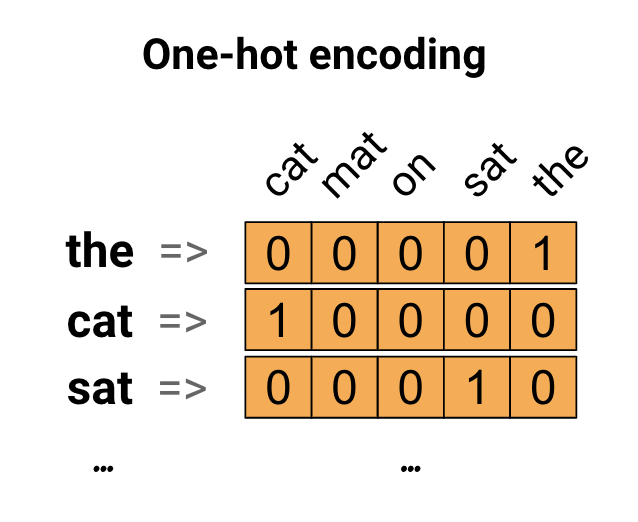
\includegraphics[width=0.5\textwidth]{Figures/one-hot.png}
	\caption{One-hot encoding~\cite{link5}}\label{fig:One-hot encoding}
\end{figure}

\subsection{Využití v praxi One-hot kódování}
V následující ukázce~\ref{src:PythonHot} je prezentována implementace metody pro konverzi lidsky psaného textu do číselných vektorů pomocí one-hot kódování.

\begin{lstlisting}[language=Python,label=src:PythonHot,caption={One-hot kódování v praxi}]
# Převod textu pomocí One-hot kódování
lidsky_text = [
	"Ja jsem nejlepsi ze vsech",
    "Ja jsem nejhorsi ze vsech"
	]

unikatni_slova = set()
for veta in lidsky_text:
    for slovo in veta.split():
        unikatni_slova.add(slovo)
    ...

slovnik = {}
for unikatni_index, unikatni_slovo in enumerate(unikatni_slova):
    one_hot_encoding_vektor = [0] * len(unikatni_slova)
    one_hot_encoding_vektor[unikatni_index] = 1
    slovnik[unikatni_slovo] = one_hot_encoding_vektor
    ...
\end{lstlisting}

V uvedené ukázce je představeno vytvoření slovníku, kde každé unikátní slovo je převedeno na číselný vektor pomocí metody one-hot kódování.
Níže~\ref{src:One-hot encoding} je příklad reprezentace několika slov ve slovníku:

\begin{lstlisting}[label=src:One-hot encoding,caption={One-hot kódování prezentace výsledného formátu dat}]
nejhorsi  : [1, 0, 0, 0, 0, 0]
ze        : [0, 1, 0, 0, 0, 0]
Ja        : [0, 0, 1, 0, 0, 0]
nejlepsi  : [0, 0, 0, 1, 0, 0]
jsem      : [0, 0, 0, 0, 1, 0]
vsech     : [0, 0, 0, 0, 0, 1]
\end{lstlisting}

\section{Vkládání slov}
Vkládání slov (word embedding) je pokročilá metoda pro převod lidsky psaného textu do číselného vektoru, která nahrazuje one-hot kódování. Tato metoda, která se využívá i v praktické části této práce, umožňuje reprezentovat slova pomocí vektorů s desetinnými čísly. Každé číslo ve vektoru reprezentuje různé vlastnosti a vztahy mezi slovy.

Pro výpočet těchto vektorů se používají různé metody, které umožňují zachytit kontext slov a jejich vztahy.
Na rozdíl od one-hot kódování, kde každé slovo má pouze jedinou hodnotu 1 ve vektoru, vkládání slov přináší bohatší informace o kontextu daného slova v textech.

Vkládání slov~\cite{link5}~\ref{fig:Word embedding} má také vlastnost vysoce dimenzionální reprezentace slov, pomocí které zachycuje kontext, ve kterém se slova vyskytují.
Tato vylepšená metoda umožňuje strojům, zpracovávající přirozený jazyk, pracovat s dodatečnými informacemi o podobnosti slov.

Díky technice vkládání slov mají stroje větší schopnost porovnávat a porozumět podobnosti mezi slovy na základě jejich kontextu. To přináší vylepšení v oblasti zpracování přirozeného jazyka a umožňuje lépe porozumět lidsky psanému textu.

\begin{figure}[H]
	\centering
	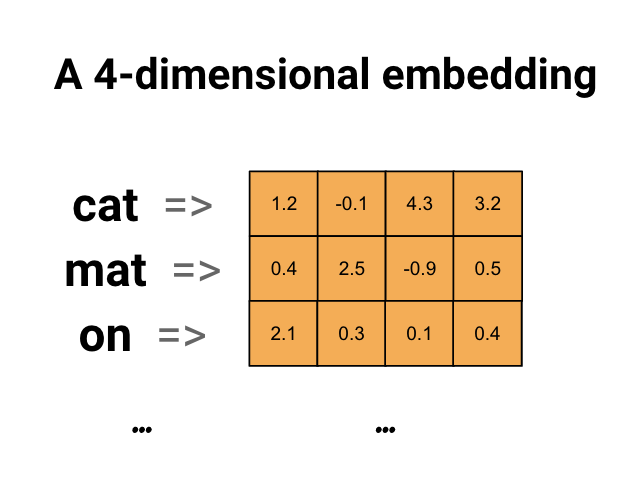
\includegraphics[width=0.6\textwidth]{Figures/embedding2.png}
	\caption{Word embedding~\cite{link5}}\label{fig:Word embedding}
\end{figure}

\subsection{Word2Vec}
Word2Vec~\cite{link6} je významným příkladem modelu pro vytváření vkládání slov~\cite{link5} a byl vyvinutý Tomášem Mikolovem z Google. Tento model umožňuje efektivní převod textu do strojové podoby a zachycuje vztahy mezi slovy.

Word2Vec~\ref{fig:Word2Vec predstaveni moznosti} se skládá z několika algoritmů, které jsou schopné naučit se reprezentaci slov. Existují dva hlavní modely pro učení techniky vkládání slov pomocí Word2Vec: Continuous Bag-of-Words (CBOW) a Continuous Skip-gram.

Continuous Bag-of-Words (CBOW) model se snaží předpovědět aktuální slovo na základě okolních slov v kontextu. Naopak, Continuous Skip-gram model se snaží na základě aktuálního slova předpovědět okolní slova v kontextu. Oba tyto modely přispěly k rozvoji výzkumu vkládání slov a převodu textu do strojové podoby.

Nicméně, i přes úspěch Word2Vec se ukázalo, že existuje efektivnější metoda, která dosahuje stejných výsledků. Tato metoda se nazývá GloVe (Global Vectors for Word Representation)~\cite{link18}. GloVe je algoritmus, který kombinuje globální statistiky slov a lokální kontextové informace při vytváření vkládání slov. Tento přístup umožňuje efektivnější a výkonnější reprezentaci slov.

GloVe se stal populární volbou pro vytváření vkládání slov díky své schopnosti zachytit vztahy mezi slovy ve velkých korpusových datech. Tato metoda přinesla další pokrok v oblasti zpracování přirozeného jazyka a významně přispěla k porozumění slov a jejich kontextu strojovými modely.

\begin{figure}[H]
	\centering
	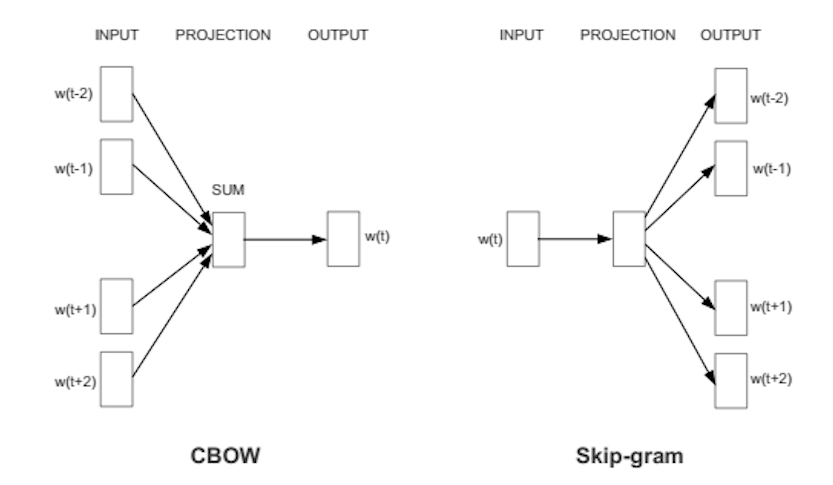
\includegraphics[width=1\textwidth]{Figures/word2vec_diagrams.png}
	\caption{Word2Vec představení možností~\cite{link6}}\label{fig:Word2Vec predstaveni moznosti}
\end{figure}

\section{GloVe}
GloVe (Global Vectors for Word Representation)~\cite{link18} je vylepšeným modelem v porovnání s Word2Vec~\cite{link6} a také vytváří reprezentaci vkládaných slov.
GloVe představuje vylepšenou verzi Word2Vec a přináší několik změn.

Hlavním rozdílem mezi GloVe a Word2Vec je, že GloVe kombinuje obě techniky, Continuous Bag-of-Words (CBOW) a Skip-gram, místo omezení na jednu z nich.
Tímto způsobem GloVe získává výhody obou přístupů.

GloVe je založen na počtu výskytů (count-based).
Tento model se učí vytvářet vkládání slov pomocí redukce dimenzí na matici počtů společných výskytů slov.
Nejprve se vytvoří velká matice, ve které jsou zachyceny informace o tom, jak často se slova vyskytují v různých kontextech ve vstupních datech.
Poté je tato matice převedena na matici nižší dimenze, kde každý řádek představuje vektorovou reprezentaci jednoho slova.

V případě GloVe je matice počtů normalizována vzhledem k počtu výskytů a následně upravena pomocí log-smoothing techniky. GloVe produkuje reprezentaci vkládaných slov, která je kontextově nezávislá, což znamená, že každé slovo je reprezentováno pouze jedním 1D vektorem, který sdružuje různé vlastnosti a vztahy tohoto slova ve vstupním textu. GloVe je také model založený na slovech (word-based), což znamená, že přijímá slova jako vstupní data a generuje vkládání slov jako výstup.

GloVe a Word2Vec se obecně podobně chovají a dosahují podobných výsledků. Výhodou GloVe je však snadnější implementace paralelizace, což vede k vyšší efektivitě.

Vytvořená reprezentace vztahů mezi jednotlivými slovy lze pochopitelněji vypozorovat z obrázku~\ref{fig:GloVe reprezentace slov ve 2D prostoru} 
\begin{figure}[H]
	\centering
	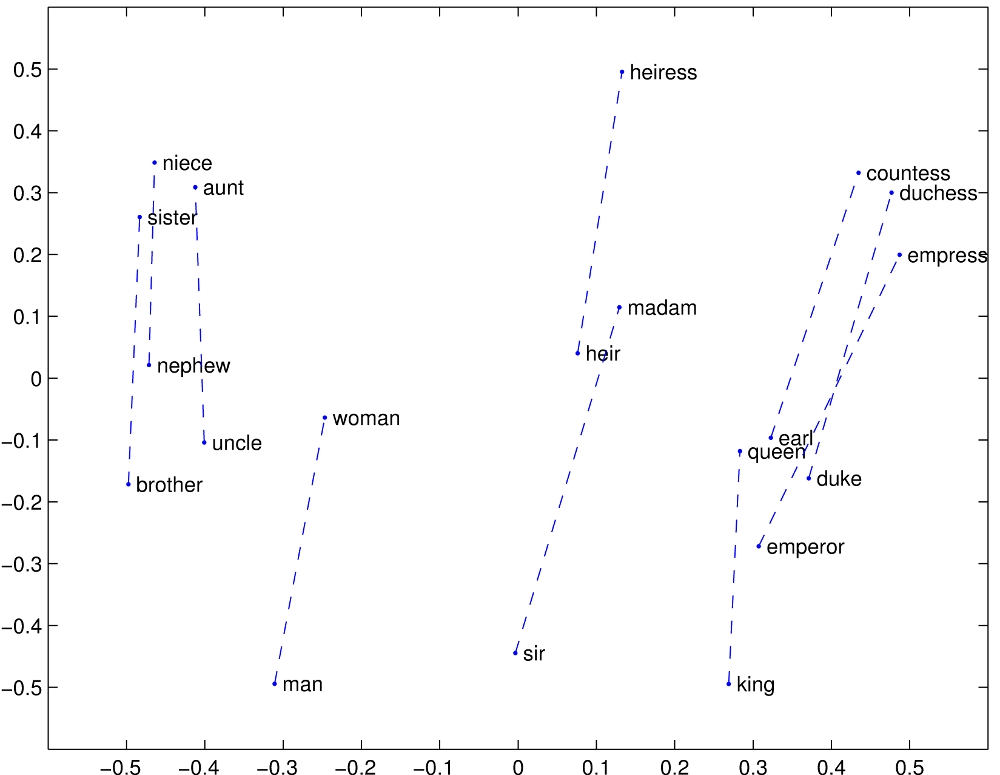
\includegraphics[width=0.8\textwidth]{Figures/GloVe_representation.jpg}
	\caption{GloVe reprezentace slov ve 2D prostoru~\cite{link18}}\label{fig:GloVe reprezentace slov ve 2D prostoru}
\end{figure}

\subsection{Continuous Bag-Of-Words}
Continuous Bag-Of-Words (CBOW)~\cite{link12} je model strojového učení používaný pro vytváření reprezentace vkládaných slov.
Jeho hlavním cílem je předpovědět cílové slovo na základě kontextu, který je definován jako určitý počet slov před a za daným slovem v textu.
CBOW se snaží naučit vektory slov, které mají kvalitní reprezentace pro předpovídání cílových slov na základě kontextuálního významu.

\subsection{Skip-gram}
Metoda Skip-gram~\cite{link13} je další volbou pro model Word2Vec a také je používána společně s CBOW v GloVe.
Hlavním rozdílem mezi Skip-gram a CBOW je v tom, co tyto metody přesně předpovídají.

CBOW předpovídá slovo na základě jeho okolí.
Zkouší určit, jaké slovo by se nejlépe hodilo do středu daného okolí na základě kontextu.
Například, pokud bylo okolí slova `auto' ve větě `Rychle jedoucí auto předjelo nákladní vozidlo' CBOW se snaží předpovědět slovo `rychle' na základě slov `jedoucí' a `předjelo'.

Na druhou stranu, metoda Skip-gram předpovídá okolí daného slova.
Zkouší určit, jaká slova by se mohla objevit v okolí daného slova na základě kontextu.
Pokračujeme-li v příkladu věty `Rychle jedoucí auto předjelo nákladní vozidlo', Skip-gram by se snažil předpovědět slova `jedoucí' a `předjelo' na základě slova `auto'.

\subsection{CBOW a Skip-gram porovnání}
V rámci modelu Word2Vec je metoda CBOW rychlejší, protože zpracovává celý kontext jako jednu entitu.

Metoda Skip-gram vytváří různé páry slov pro každé slovo v kontextu.
Každý pár se skládá z jednoho vstupního centrálního slova a jednoho výstupního okolního slova.
Skip-gram se snaží předpovědět okolní slova na základě daného centrálního slova.

Nicméně, výběr mezi metodou CBOW a Skip-gram závisí na konkrétních úkolech a datových sadách.
Obě metody mají své výhody a omezení a jejich volba závisí na konkrétních potřebách a podmínkách aplikace.

\endinput